\documentclass{beamer}
\usepackage[utf8]{inputenc}

\title{Matrix Project}
\author{EE17BTECH11023 \and EE17BTECH11007}

\usetheme{AnnArbor}
\begin{document}

\section{Introduction to AI and ML}
\maketitle

\begin{frame}{Geometry Question:}
Two sides of a rhombus are along the lines,
x – y + 1 = 0 and 7x – y – 5 = 0. If its diagonals
intersect at (–1, –2), then which one of the
following is a vertex of this rhombus.
Find its vertices.\\
(Q 13 JEE MAINS CODE-G)

    
\end{frame}

\begin{frame}{Question in Matrix form:}

Two sides of a rhombus are along the lines\\
$ \begin{bmatrix}
  \ 1 &\ -1 \\
\end{bmatrix}
\textbf{x} + 1 = 0 $ \\ 
$  \begin{bmatrix}
  \ 7 &  \ -1 \\
\end{bmatrix} \textbf{x} - 5 = 0 $\\
If its diagonals intersect at
$ 
\begin{bmatrix}
  \ -1 \\
  \ -2 \\
\end{bmatrix}
$
.Find its vertices.\\
(Q26 in jee-linalg-2d)

    
\end{frame}

\begin{frame}{Solution Approach:}
Since we are given 2 sides of rhombus \textbf{L1}, \textbf{L2} we will get a vertex \textbf{A} of rhombus from intersection of the given lines.\\
We also know the point of intersection of diagonals, \textbf{O}, thus we now know the equation of diagonal \textbf{D1}  through \textbf{O} and \textbf{A}.
Since we know the equation of the diagonal, we know the vertex \textbf{B} opposite to \textbf{A} because \textbf{O} is the midpoint of \textbf{A} and \textbf{B}.\\As we know the equation of the diagonal \textbf{D1} passing through \textbf{A}\textbf{B} we can find the equation of other diagonal \textbf{D2} which is perpendicular to the former and passing through \textbf{O} (by the property of Rhombus). Now we can find another vertices \textbf{C} and \textbf{D} which are the intersections of the diagonal \textbf{D2} with each of the given lines or we can find one point using this method and the other using the same method as used for finding \textbf{B}.
    
\end{frame}

\begin{frame}{Method to find intersection of two lines:}
Let the respective equations be\\
$\textbf{n}^T_1 \textbf{x} = p_1 $\\ $\textbf{n}^T_2 \textbf{x} = p_2 $\\

This can be written as the matrix equation \\
$ \begin{bmatrix}
  \ \textbf{n}^T_1 \\
  \ \textbf{n}^T_2 \\
\end{bmatrix} $
$ \textbf{x} = \textbf{p} $\\
$ N^T \textbf{x} = \textbf{p} $\\

where
 N = $\begin{bmatrix}
 \textbf{n}_1 &\
 \textbf{n}_2 
\end{bmatrix} $ \\

The point of intersection is then obtained as
$\textbf{x} = (N^T)^{-1} \textbf{p}$ \\
$\textbf{x}= N^{-T}\textbf{p}$


\end{frame}

\begin{frame}{Method to find intersection of two lines(calculations):}
We use this method to find \textbf{A} from intersection of \textbf{L1} and \textbf{L2}\\
$\textbf{n}_1^T $=$\begin{bmatrix}
  \ 1 &\ -1 \\
\end{bmatrix} $
\\
 
 $\textbf{n}_2^T$=$\begin{bmatrix}
  \ 7 &\ -1 \\
\end{bmatrix} $\\
$N^T$=$\begin{bmatrix}
  \ 1 &\ -1 \\
  \ 7 &\ -1 \\
\end{bmatrix}$ \\ 
 $N^{-T}$=$\begin{bmatrix}
  \ -1/6 &\ 1/6 \\
  \ -7/6 &\ 1/6 \\
\end{bmatrix} $\\

\textbf{p}= $\begin{bmatrix}
  \ -1 \\ 5 \\
\end{bmatrix} $ \\

\textbf{A}=$ N^{-T} $ \textbf{p}=$ \begin{bmatrix}
  \ 1 \\ 2 \\
\end{bmatrix} $ \\

And \textbf{C} and \textbf{D} from intersection of \textbf{L1} and \textbf{L2} with \textbf{D2}


\end{frame}

\begin{frame}{Method to find intersection of two lines(calculations):}
We use this method to find \textbf{C} from intersection of \textbf{L1} or \textbf{L2} with \textbf{D2}\\
for \textbf{L1}\\ 
$\textbf{n}_1^T$ = $
\begin{bmatrix}
  \ 1 &\ -1 \\
\end{bmatrix} $ \\
$ p1=-1 $\\
for \textbf{D2}\\ 
\textbf{n}d is directional vector of \textbf{D1}, which is equal to \textbf{O-A}\\
$\textbf{n}d^T$=$\begin{bmatrix}
  \ -2 &\ -4 \\

\end{bmatrix}$ \\
  pd=$\textbf{n}d^T$ $\textbf{O}=10$\\
  
  $N^T$=$\begin{bmatrix}
  \ 1 &\ -1 \\
  \ -2 &\ -4 \\
\end{bmatrix}$ \\
$N^{-T}$=$\begin{bmatrix}
  \ 2/3 &\ -1/6 \\
  \ -1/3 &\ -1/6 \\
\end{bmatrix}$ \\
\textbf{p}=$\begin{bmatrix}
  \ -1 \\ 10 \\
\end{bmatrix}$ \\

\textbf{C}=$ N^{-T} $ \textbf{p}=$\begin{bmatrix}
  \ -2.33333333 \\ -1.33333333 \\
\end{bmatrix}$

 
\end{frame}

\begin{frame}{Method using midpoints:}
If \textbf{O} is the midpoint of \textbf{A} and \textbf{B}\\
\textbf{O}=(\textbf{A}+\textbf{B})/2\\
\textbf{B}=2\textbf{O}-\textbf{A}\\
\textbf{B}=\textbf{A}+2(\textbf{O-A})
We know that the diagonals in a Rhombus bisect each other\\
\textbf{O} is the midpoint of opposite vertices of the Rhombus\\
Thus given \textbf{O} and \textbf{A} we can find \textbf{B}\\

\textbf{B}=\textbf{A}+2(\textbf{O-A})=$\begin{bmatrix}
  \ -3 \\ -6 \\

\end{bmatrix} $\\

And given \textbf{O} and either of \textbf{C} or \textbf{D} we can find the other.\\


\textbf{D}=\textbf{C}+2(\textbf{O-C})=$\begin{bmatrix}
  \  0.33333333 \\ -2.66666667 \\

\end{bmatrix} $

\end{frame}

\begin{frame}{Graph}
\centering
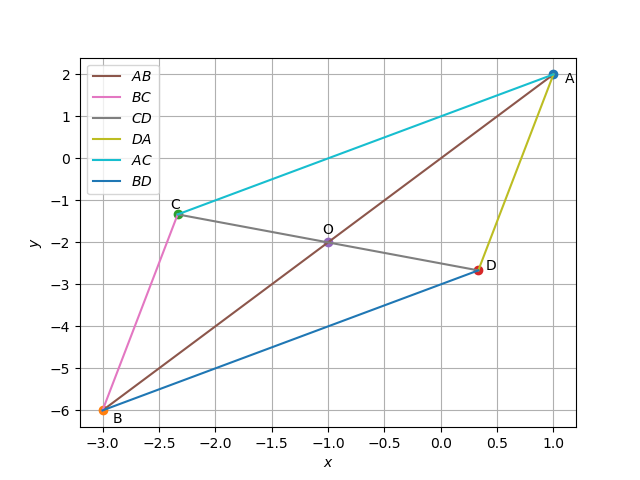
\includegraphics[scale=0.6]{Figure_1.png}
    
\end{frame}

\end{document}
